\documentclass[margin=10pt]{standalone}
\usepackage{tikz}
\usetikzlibrary{calc} % for coordinate arithmetic
\usepackage{xcolor}

% --- Colors for genes ---
\definecolor{gene1}{RGB}{228,26,28}
\definecolor{gene2}{RGB}{55,126,184}
\definecolor{gene3}{RGB}{77,175,74}
\definecolor{gene4}{RGB}{152,78,163}
\definecolor{gene5}{RGB}{255,127,0}

% --- Unique genes in order (IR duplicates removed) ---
% Format: start/stop/color/label
\def \LinearGenes{%
10/40/gene1/Gene1,%
70/110/gene2/Gene2,%
140/180/gene3/Gene3,%
205/230/gene4/Gene4,%
240/265/gene5/Gene5}

% --- Scale: bp -> physical length (set to taste) ---
\newcommand{\Scale}{0.05cm} % each 1 bp becomes 0.05 cm of width

\begin{document}
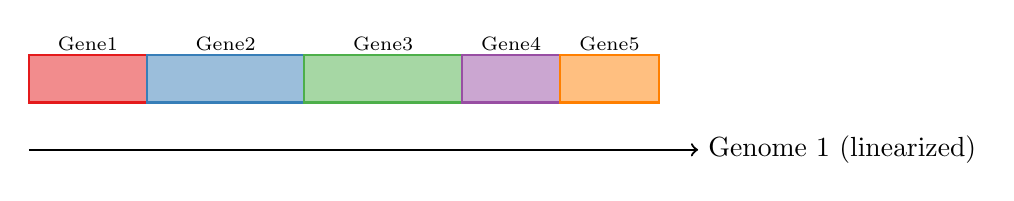
\begin{tikzpicture}

% Starting reference point for the first gene
\coordinate (p0) at (0,0);

% Draw each gene consecutively (no overlaps)
\foreach \s/\t/\col/\lab [count=\i] in \LinearGenes {%
  % width as a length (safe arithmetic with units)
  \pgfmathsetlengthmacro{\w}{(\t-\s)*\Scale}%
  % next endpoint coordinate = previous + (width, 0)
  \coordinate (p\i) at ($ (p\the\numexpr\i-1\relax) + (\w,0) $);
  % draw the gene rectangle from previous to current
  \path[draw=\col, fill=\col!50, thick]
    ($ (p\the\numexpr\i-1\relax) + (0,0.3) $)
      rectangle
    ($ (p\i) + (0,0.9) $);
  % label at midpoint between previous and current
  \node[font=\scriptsize, align=center]
    at ($ (p\the\numexpr\i-1\relax)!0.5!(p\i) + (0,1.05) $) {\lab};
  % remember the running end point
  \coordinate (plast) at (p\i);
}

% Axis line under the genes
\draw[thick,->] (0,-0.3) -- ($ (plast) + (0.5cm,-0.3) $) node[right]{Genome 1 (linearized)};

\end{tikzpicture}
\end{document}
